 %----------------------------------------------------------------------------------------
%	PACKAGES AND DOCUMENT CONFIGURATIONS
%----------------------------------------------------------------------------------------
\documentclass[11pt]{article}
\usepackage{subcaption}
\usepackage{amsmath} % Required for some math elements
\usepackage{hyperref} 
\usepackage[table,xcdraw]{xcolor}
\usepackage{lipsum} 
\usepackage{cite}
\usepackage{graphicx} % Required for the inclusion of images
\usepackage{algorithmic}
\usepackage{array}
\usepackage{bookmark}
\usepackage{listings}
\usepackage{amssymb}
\usepackage{enumitem}
\usepackage{pythonhighlight}
\usepackage[T1]{fontenc}
\usepackage{inconsolata}
\usepackage[margin=16mm]{geometry}
\usepackage{cleveref}

\newlist{steps}{enumerate}{1}
\setlist[steps, 1]{label = Step \arabic*:}

\hypersetup{ %color attributes of citation, link, etc.
    colorlinks=true,
    linkcolor=blue,
    filecolor=gray,      
    urlcolor=blue,
    citecolor=blue,
}

\newcommand{\matlab}{\textsc{Matlab }} %very important and totally necessary addition
\newcommand{\hdotrule}[1]{\hbox to \textwidth{\leaders\hbox to #1pt{\hss . \hss}\hfil}}

\newcommand\Item[1][]{%
  \ifx\relax#1\relax  \item \else \item[#1] \fi
  \abovedisplayskip=0pt\abovedisplayshortskip=0pt~\vspace*{-\baselineskip}}
%----------------------------------------------------------------------------------------
%	DOCUMENT INFORMATION
%----------------------------------------------------------------------------------------


\title{ECEN 405 -  D Class Amplifier \\ \large{\textit{``What a buck convertor would say if it could talk''}} }
\author{Daniel Eisen : 300447549 \\Team members: Niels Clayton \& Nickolai Wolfe}
\date{}

\begin{document}
\maketitle
\begin{center}
  \vspace*{-8mm}
  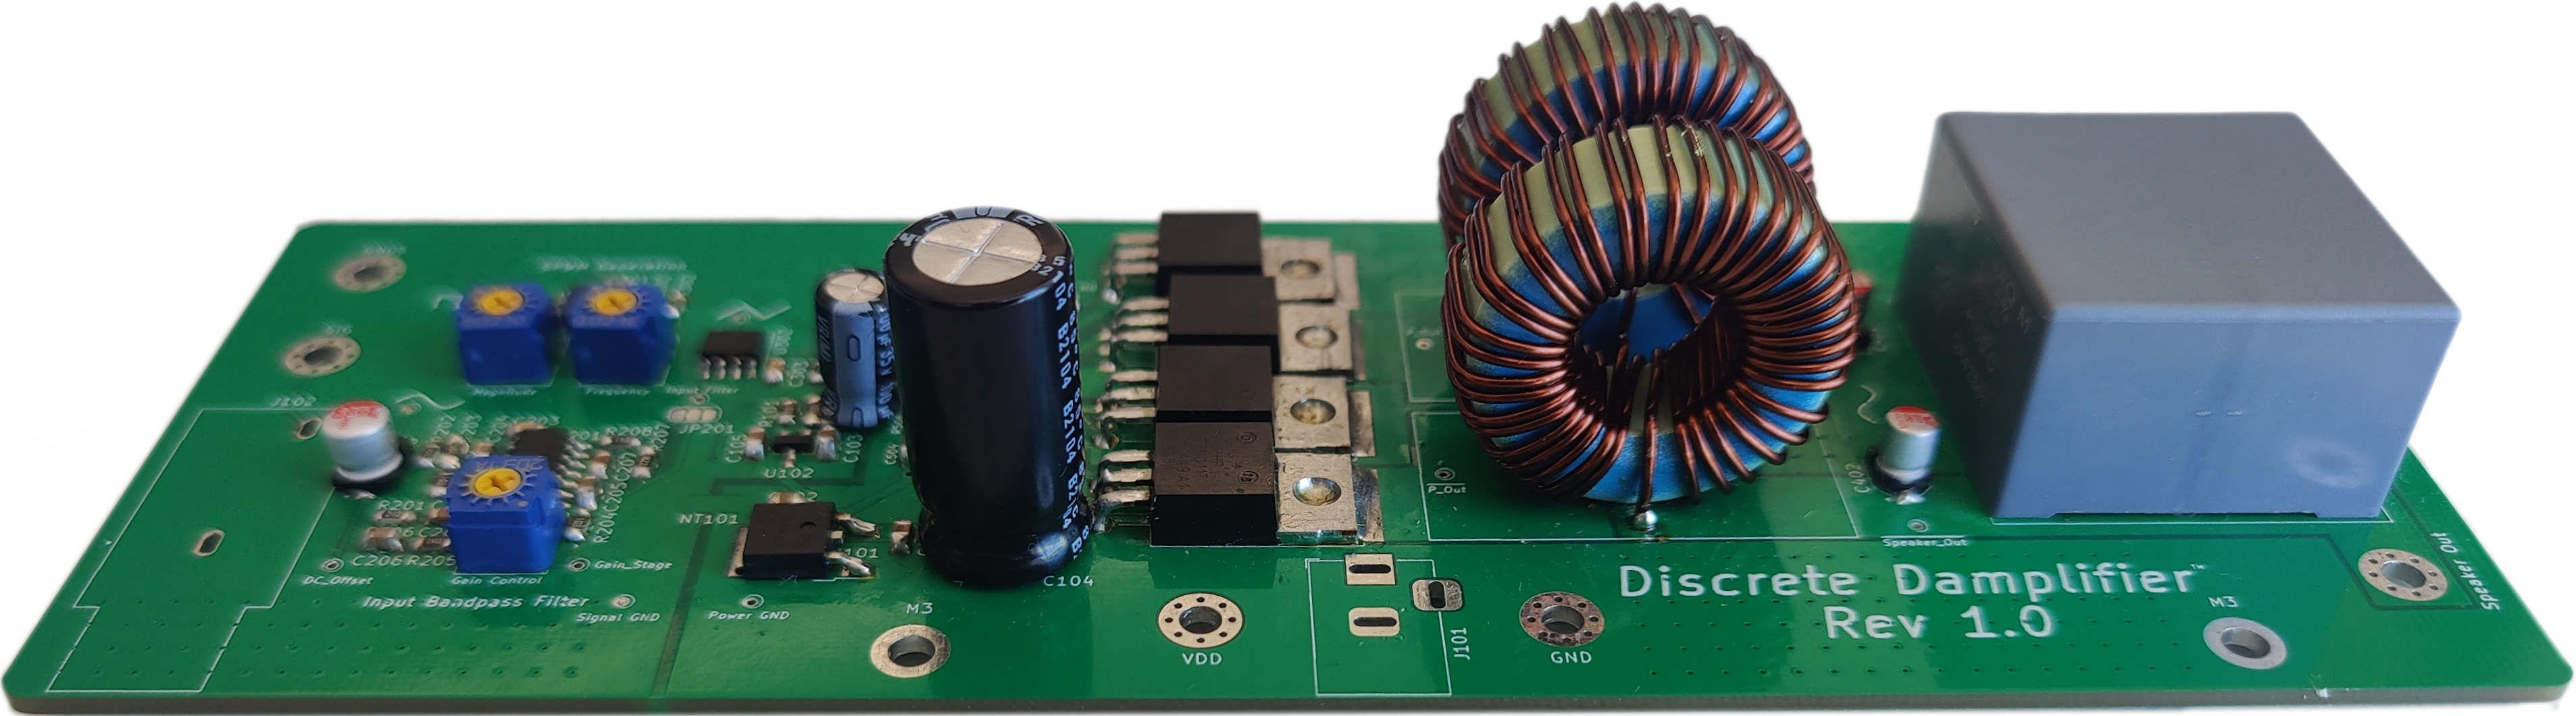
\includegraphics[width=0.75\textwidth]{img/real.png}
\end{center}{

\section{Introduction}

In the relm of auido ampliifers the D Class offers a method of supplying a high power loads with very high efficiency (esspecailly when compared to other classes). Classes A, AB offer high power output with very low signal distortion but suffer greatly in the efficency department due to continous linear conduction times and resulting losses in their amplifying elements/transistors. D class amplifiers can achieve up to 90-95\% power efficiency by taking advantage of a switching approach but require a more complex design process and circuit.

\begin{figure}[h!]
  \centering
  \frame{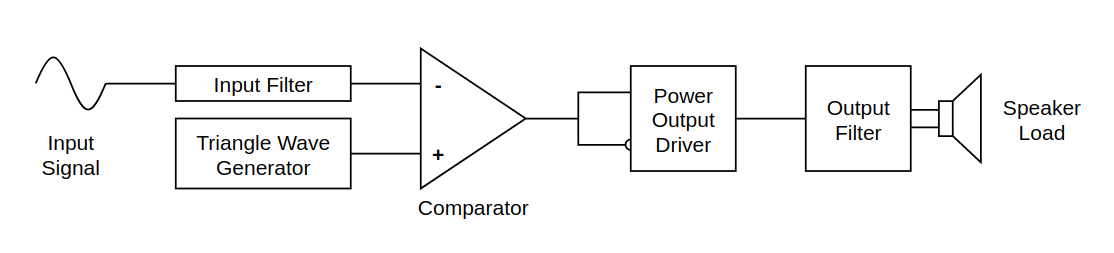
\includegraphics[width=0.8\textwidth]{img/D-class_block.png}}
  \caption{General Block Diagram of a D Class Amplifier}
  \label{F:block}
\end{figure}
A D class design can be broken up into and explain with a series of blocks illustrated above in \cref{F:block}. An input signal is sampled with a triangular wave into a high frequency SPWM carrier signal that is then amplified to high power by switching a MOSFET bridge and the carrier frequency is removed with a low pass filter. As the switching elements are either ON or OFF the continuous conduction losses near eliminated*.

This report outlines and discussed the specifics in design, implementation and results of constructing a D-class amplifier project to the specifications outlined below in \cref{S:spec}.

\subsection*{Specifications}\label{S:spec}
\begin{itemize}
  \item $P_{out}=80W$ for $R_{L} = 4\Omega$
  \item 10Hz to 200Hz Bandwidth
  \item Input sensitivity of 1V for maximum output (interpreted as 1V amplitude, 2V pk-pk)
  \item Maximum costs: \$50 per person
\end{itemize}

\section{Design}

A D-class amplifier operates on the signal sampling, switching amplification, and signal reconstruction as briefly described above. This can be practically realised \dots

Nick designed input stage that handles signal preconditioning and bandpass filtering

Niels designed Sampler and SPWM generation

I designed Power Driving Stage (Bridges) and Low Pass Output/Reconstruction filter


\begin{figure}[h!]
  \centering
  \frame{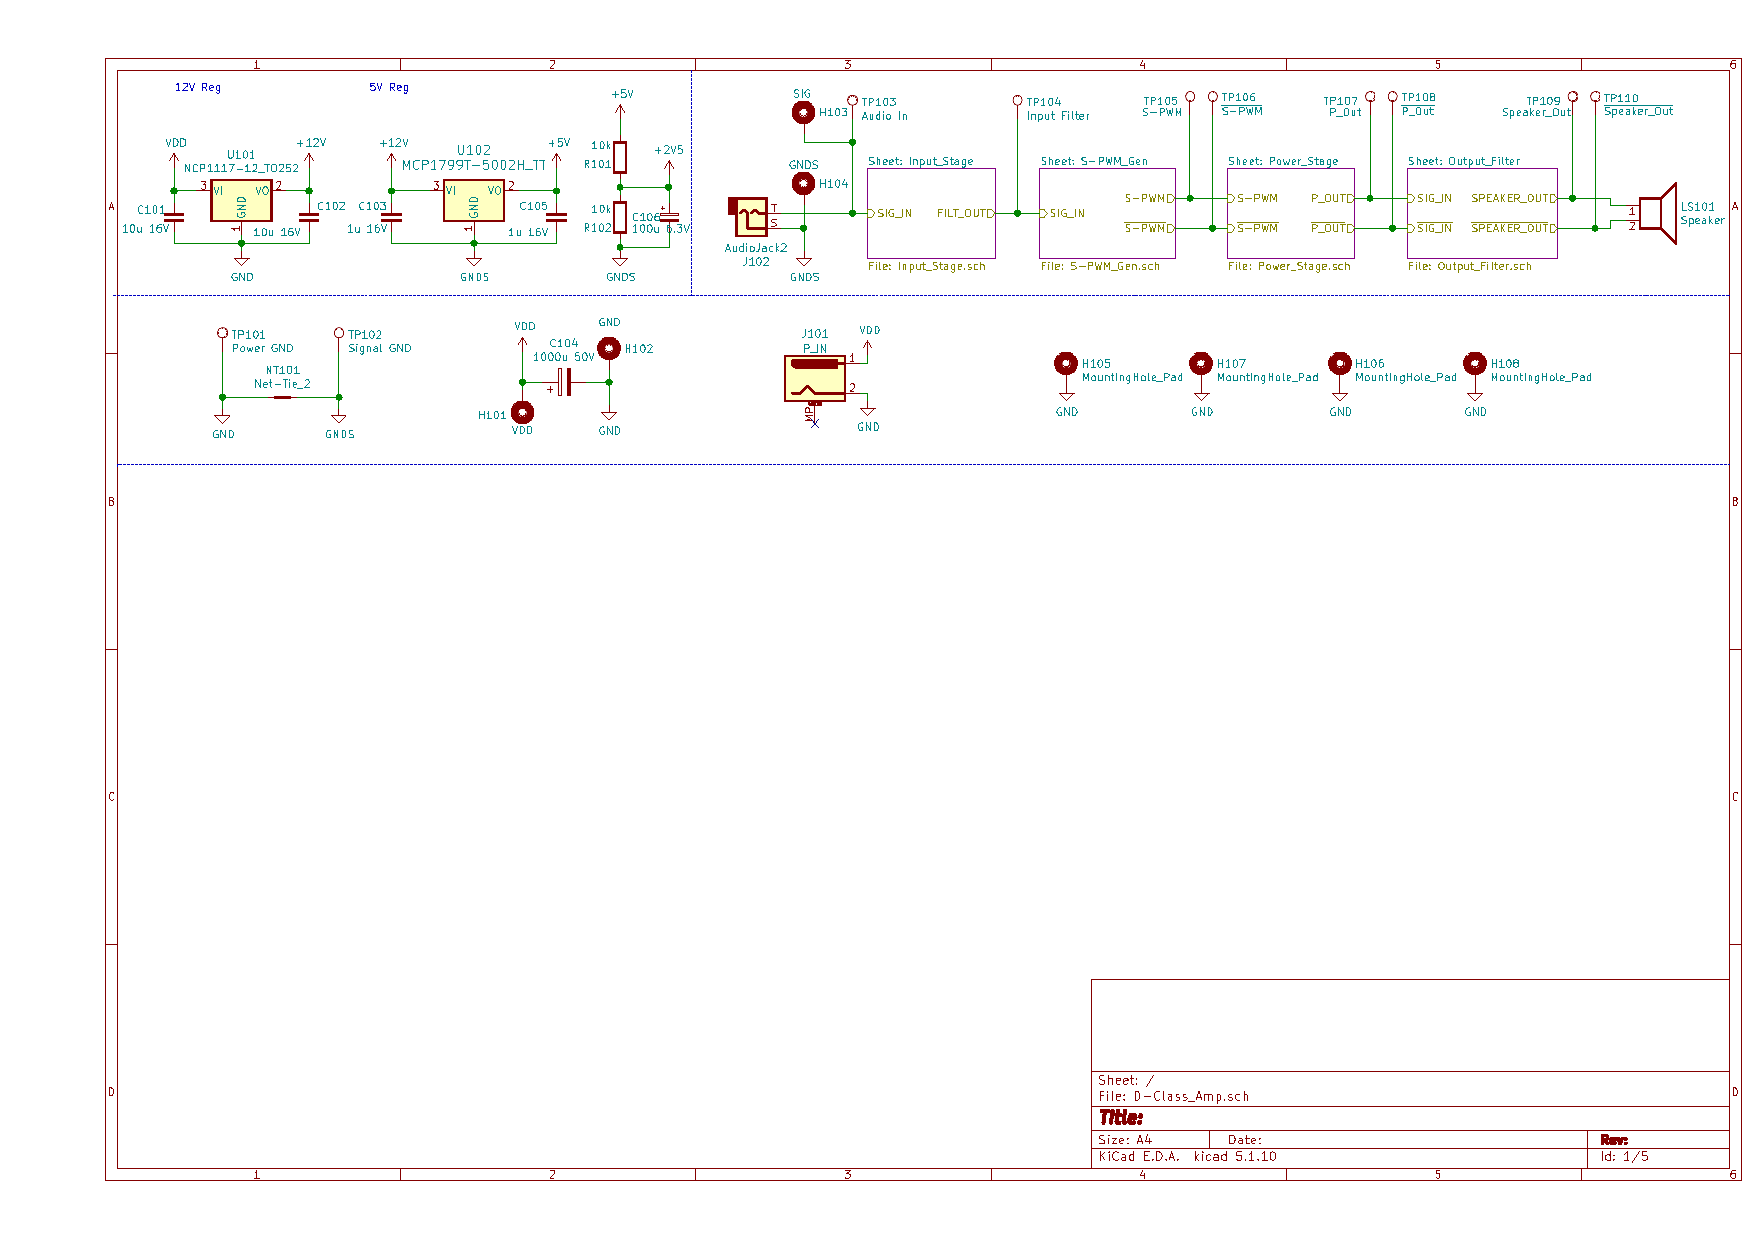
\includegraphics[page=1, trim={20mm 132mm 4.5mm 12.5mm},clip,width=0.85\textwidth]{img/schematic.pdf}}  \caption{Top Level Design Schematic}
  \label{F:top_schem}
\end{figure}

\subsection{Top Level Design Decisions}

\begin{itemize}
  \item Single main supply voltage regulated down to driver and logic supplied to produce a more cohesive final product
\end{itemize}

\begin{align*}
  V_{DD} &= \sqrt{2\cdot R_{L}\cdot P_{out}} \\
         &= 25.298V\\
  V_{DD} &= 26V (min)
\end{align*}


\subsection{Input Bandpass Filter}

Active Bandpass filter with adjustable gain stage to pass 10Hz to 200Hz.

\textit{this is what is was designed to do to meet these spec with this method, with these nice additions}

\begin{figure}[h!]
  \centering
  \frame{\includegraphics[page=2, trim={25mm 70mm 90mm 60mm},clip,width=0.85\textwidth]{img/schematic.pdf}}
  \caption{Input filtering schematic}
  \label{F:ipf_schem}
\end{figure}

\subsection{Audio Sampling and SPWM}

\begin{figure}[h!]
  \centering
  \frame{\includegraphics[page=3, trim={35mm 133.5mm 30mm 15mm},clip,width=0.85\textwidth]{img/schematic.pdf}}
  \caption{Sampling triangle wave \& SPWM generation schematic}
  \label{F:sample_schem}
\end{figure}

\subsection{Power Stage and Output Filter}

\begin{figure}[h!]
  \centering
  \frame{\includegraphics[page=5, trim={85mm 149mm 5mm 12mm},clip,width=0.85\textwidth]{img/schematic.pdf}}
  \caption{Gate driver schematic}
  \label{F:gate_drive_schem}
\end{figure}



Signal freq max of 200Hz, Switching frequency of ~30kHz
Place corner frequency of filter at 3kHz (decade centred)
mes


https://datasheets.maximintegrated.com/en/ds/MAX4295.pdf

Figure 4c. Alternate Balanced 2-Pole Filter

Balanced 2-Pole (Figure 4b):
A  balanced  2-pole  filter  does  not  have  the  common-
mode swing problem of the single-ended filter.
C = 2 / (√2 ✕ RL ✕ ωo), L = (√2 ✕ RL)/(2 ✕ ωo); choosing
fo =  3kHz  and  RL =  4Ω,  C1a  =  C1b  =  1.87μF,  L1a  =
L1b = 150μH.
A single capacitor connected across RL, with a value of
CL = 1/(√2 ✕ RL ✕ ωo), can be used in place of C1a and
C1b.  However,  the  configuration  as  shown  gives  an
improved  rejection  to  common-mode  signal  compo-
nents  of  OUT+_  and  OUT-_.    If  the  single  capacitor
scheme is used, additional capacitors (Ca and Cb) can
be  added  from  each  side  of  RL,  providing  a  high-fre-
quency  short  to  ground  (Figure  4c).  These  capacitors
should be approximately 0.2 ✕ CL.

\begin{figure}[h!]
  \centering
  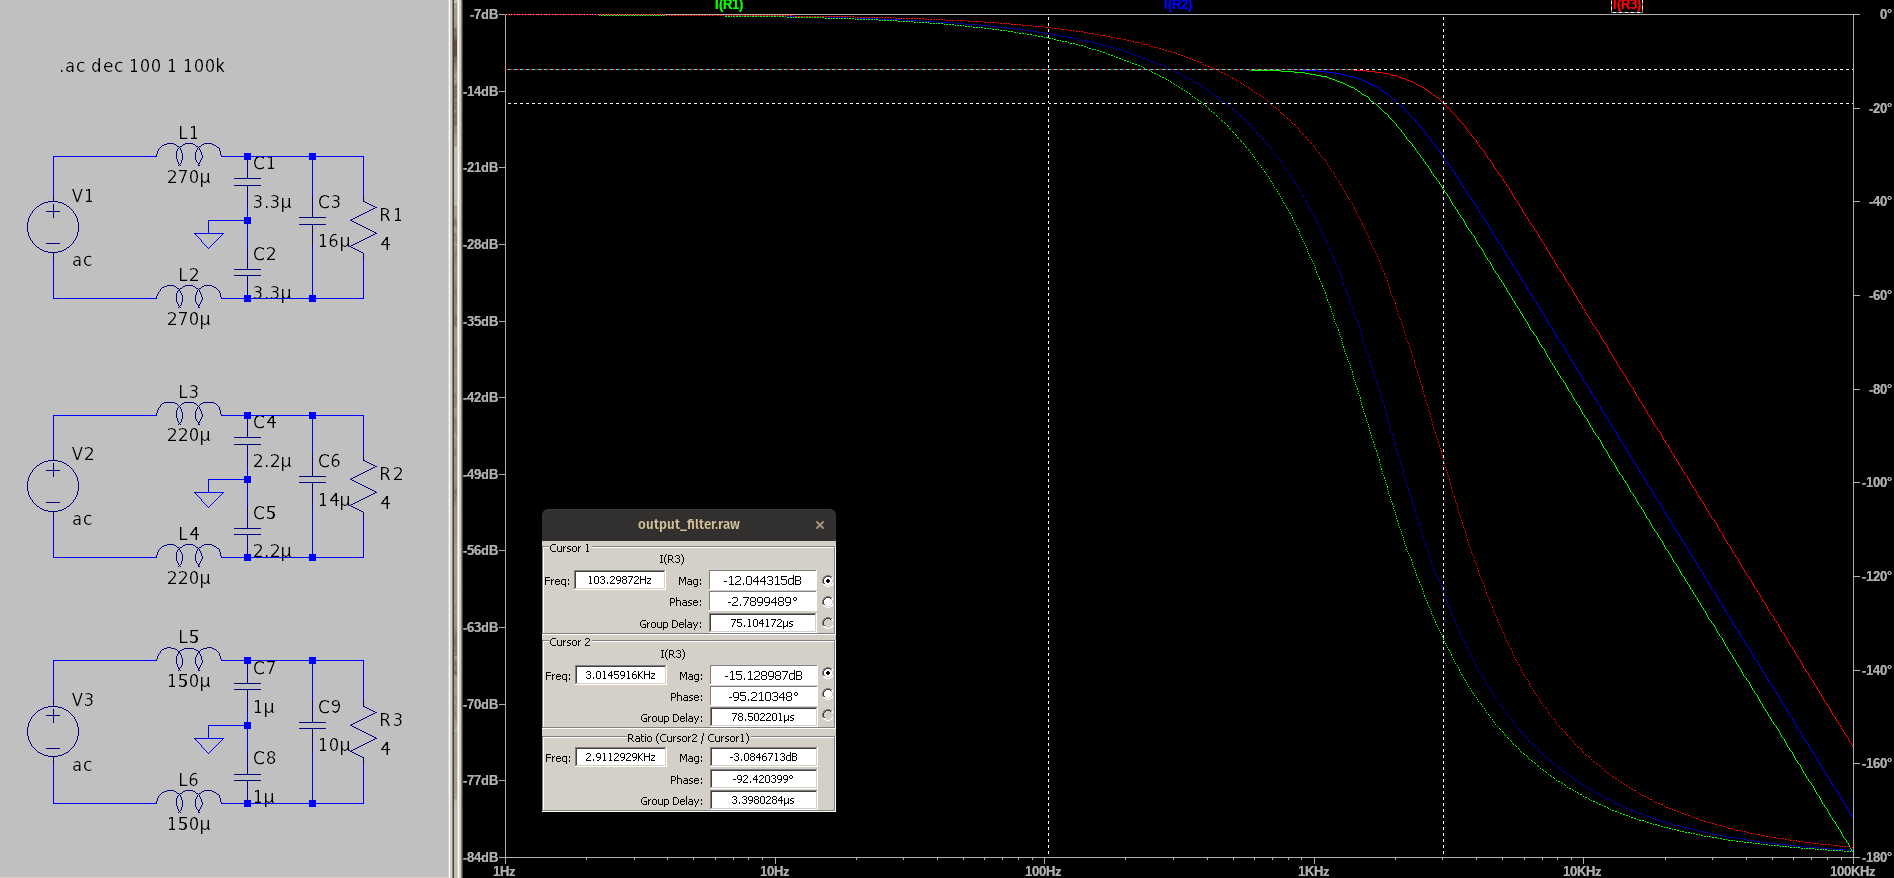
\includegraphics[width=0.75\textwidth]{img/output_filter_sim.png}
  \caption{Output filter option simulations}
  \label{F:opf_sim}
\end{figure}

\begin{figure}[h!]
  \centering
  \frame{\includegraphics[page=4, trim={115mm 97mm 105mm 75mm},clip,width=0.6\textwidth]{img/schematic.pdf}}
  \caption{Final output filter schematic}
  \label{F:opf_schem}
\end{figure}


\section{Implementation}

\textit{Here you should discuss the assembly of the amplifier and any problems you faced as a team building the amplifier.
Here, the individual components should also be characterised. For example: if you have a filter, what is the response and how does it compare to the calculated? If you have a triangle wave, how does it look? Is it doing what I should? Why? Why not? How do the inputs/outputs of your comparator look? How does the square wave on the gate of the MOSFETs look?}
 

\subsection{PCB Layout}

\begin{figure}
  \centering
  \begin{subfigure}{0.5\textwidth}
    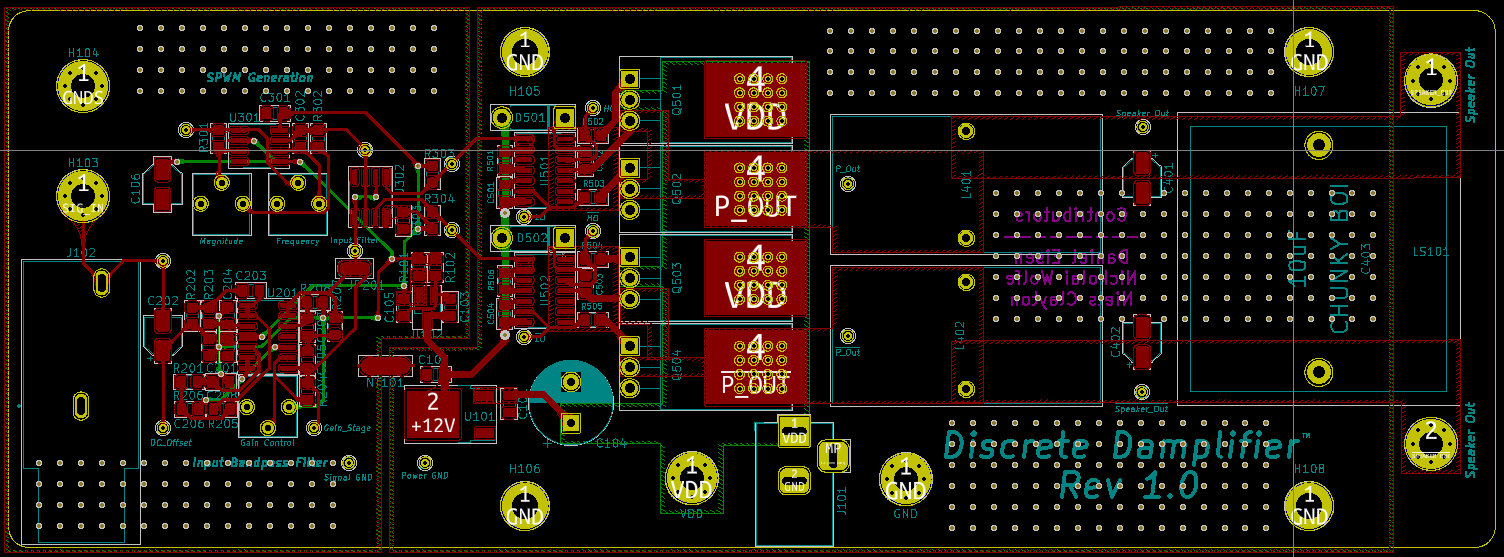
\includegraphics[width=\columnwidth]{img/traces.png}
    \subcaption{}
  \end{subfigure}
  \begin{subfigure}{0.5\textwidth}
    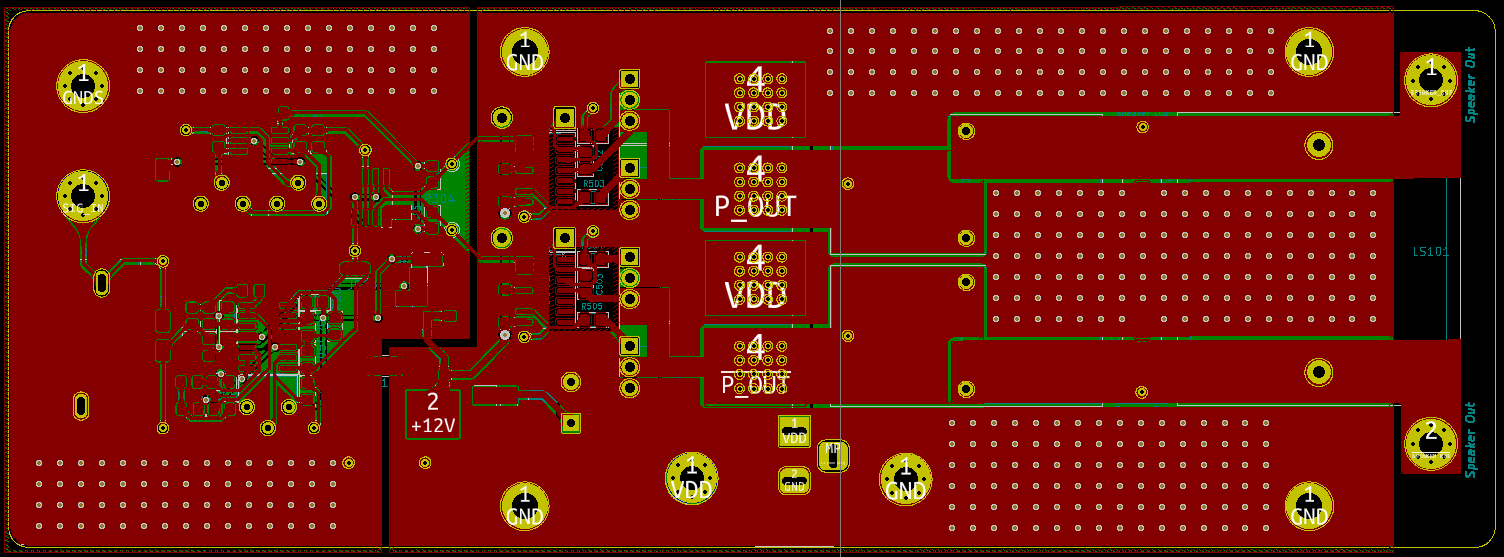
\includegraphics[width=\columnwidth]{img/top_layer.png}
    \subcaption{}
  \end{subfigure}
  \begin{subfigure}{0.5\textwidth}
    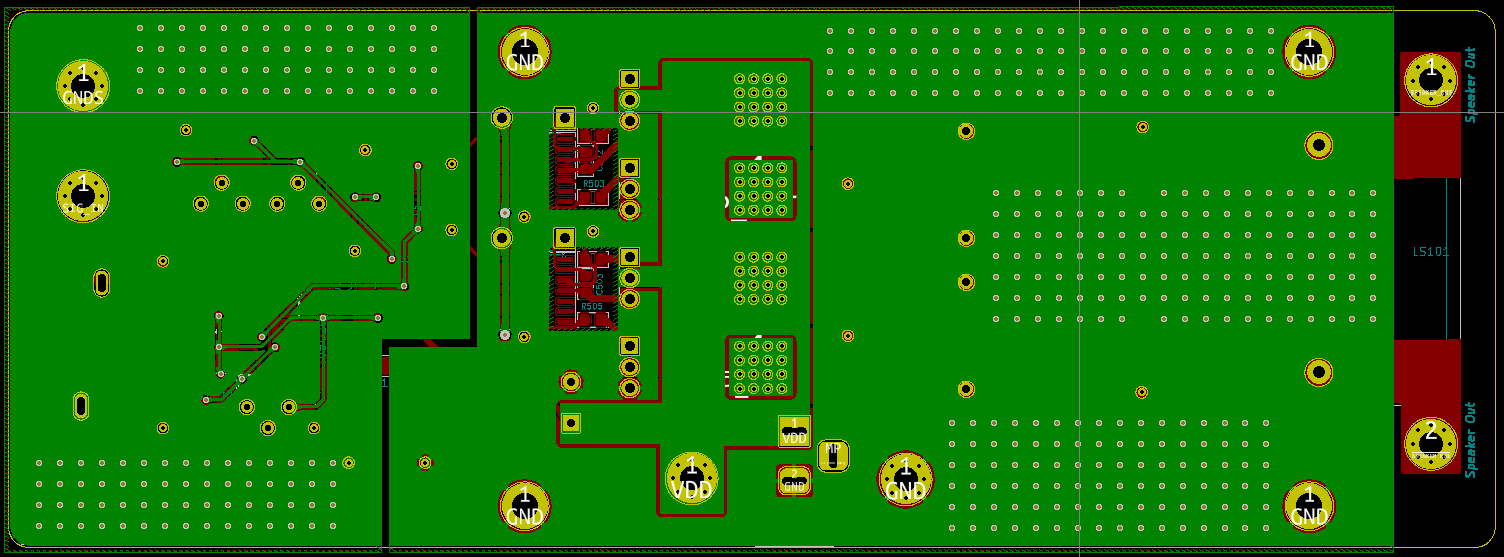
\includegraphics[width=\columnwidth]{img/bottom_layer.png}
    \subcaption{}
  \end{subfigure}
  \caption{}
\end{figure}

\subsection{Gate Driving and Bridge Output}
\begin{figure}[h!]
  \centering
  \begin{subfigure}{0.3\textwidth}
      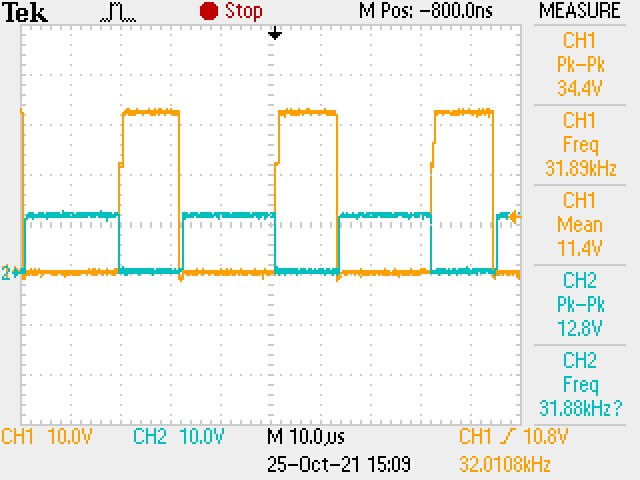
\includegraphics[width=\columnwidth]{img/testing/power_output/gate_input.JPG}
      \subcaption{High and Low side gate signals}
  \end{subfigure}
  \begin{subfigure}{0.3\textwidth}
      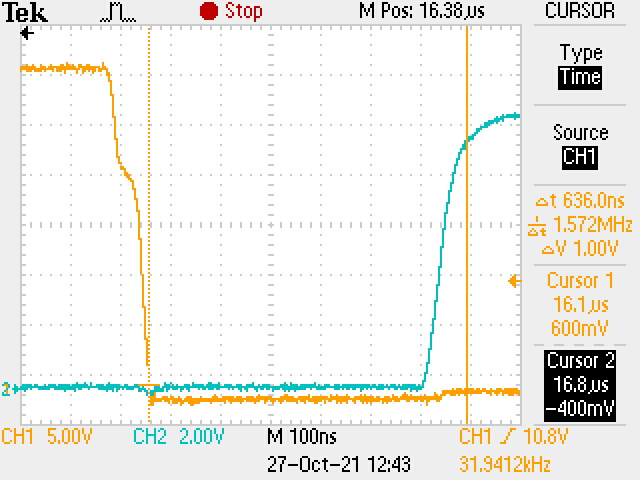
\includegraphics[width=\columnwidth]{img/testing/power_output/dead_time.JPG}
      \subcaption{Deadtime}
  \end{subfigure}
  \begin{subfigure}{0.3\textwidth}
      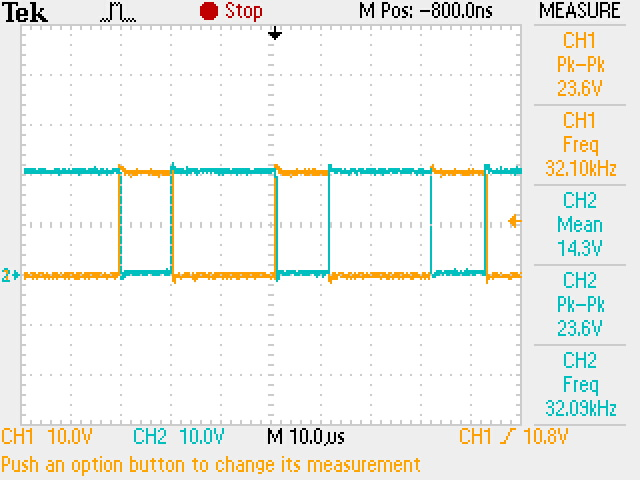
\includegraphics[width=\columnwidth]{img/testing/power_output/fet_output.JPG}
      \subcaption{Both bridges amplified SPWM (FET outputs)}
  \end{subfigure}
  \caption{}
\end{figure}


\section{Results}
 
\textit{Here I would expect to see the results of the whole amp, for example: an output wave, analysis of the efficiency, discuss maximum power output (which may be frequency dependent), and THD.} 
 
\begin{figure}[h!]
  \centering
  \begin{subfigure}{0.3\textwidth}
      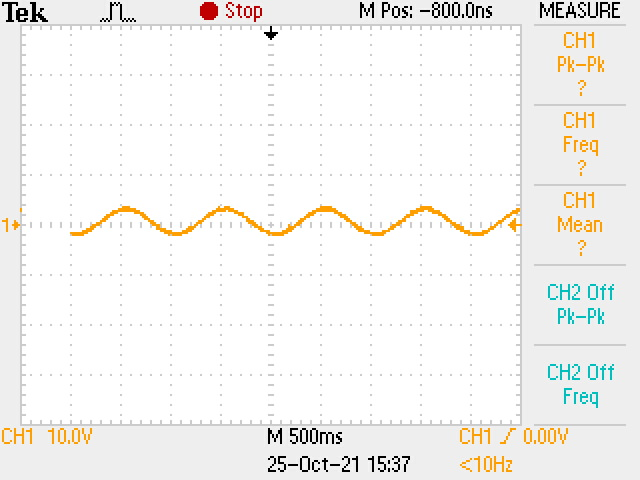
\includegraphics[width=\columnwidth]{img/testing/power_output/filter_output_1Hz.JPG}
      \subcaption{}
  \end{subfigure}
  \begin{subfigure}{0.3\textwidth}
      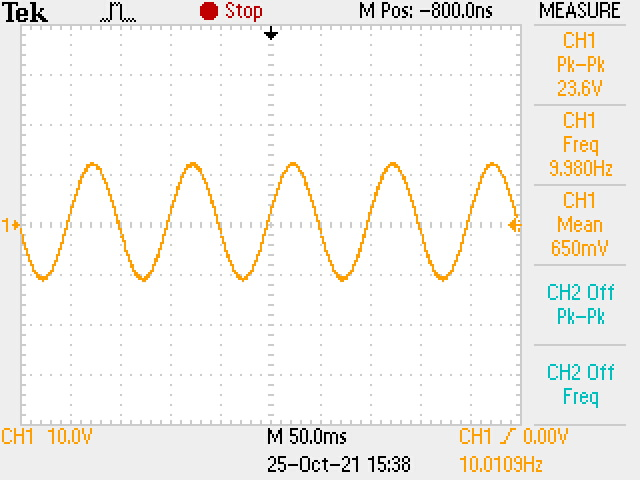
\includegraphics[width=\columnwidth]{img/testing/power_output/filter_output_10Hz.JPG}
      \subcaption{}
  \end{subfigure}
  \begin{subfigure}{0.3\textwidth}
      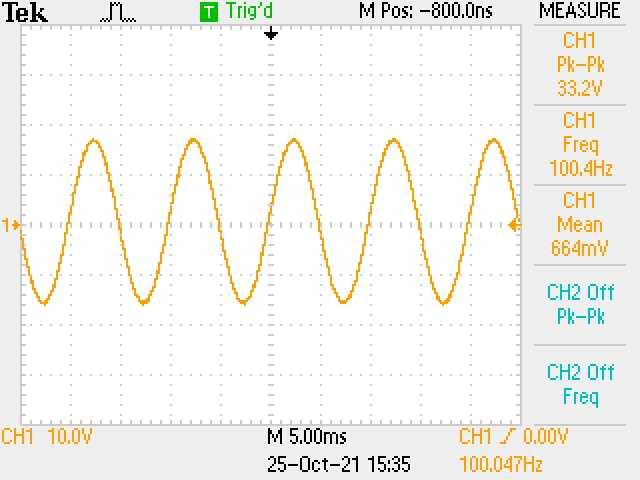
\includegraphics[width=\columnwidth]{img/testing/power_output/filter_output_100Hz.JPG}
      \subcaption{}
  \end{subfigure}
  \begin{subfigure}{0.3\textwidth}
      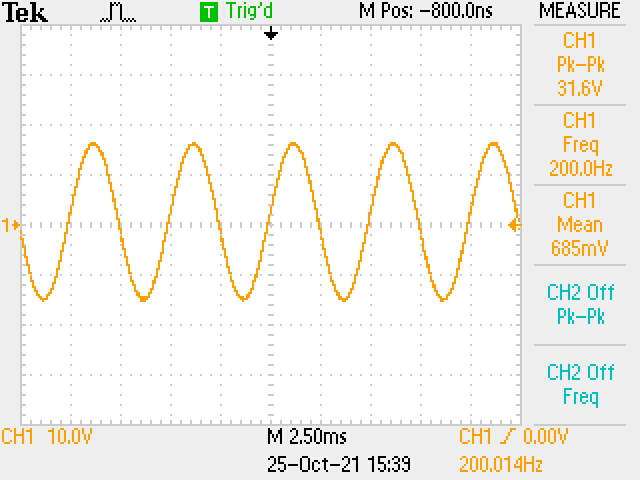
\includegraphics[width=\columnwidth]{img/testing/power_output/filter_output_200Hz.JPG}
      \subcaption{}
  \end{subfigure}
  \begin{subfigure}{0.3\textwidth}
      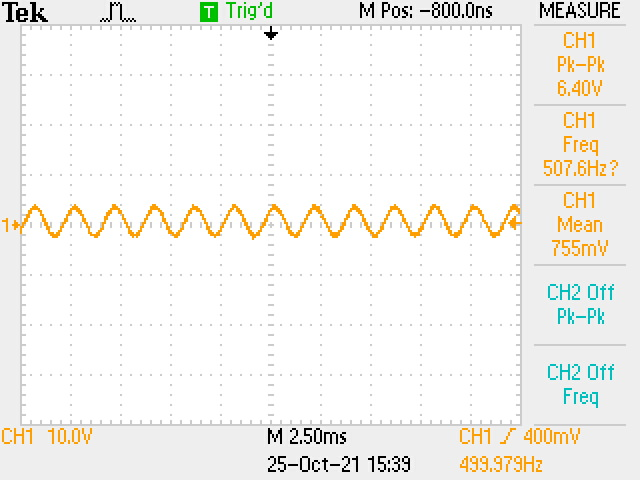
\includegraphics[width=\columnwidth]{img/testing/power_output/filter_output_500Hz.JPG}
      \subcaption{}
  \end{subfigure}
  \begin{subfigure}{0.3\textwidth}
      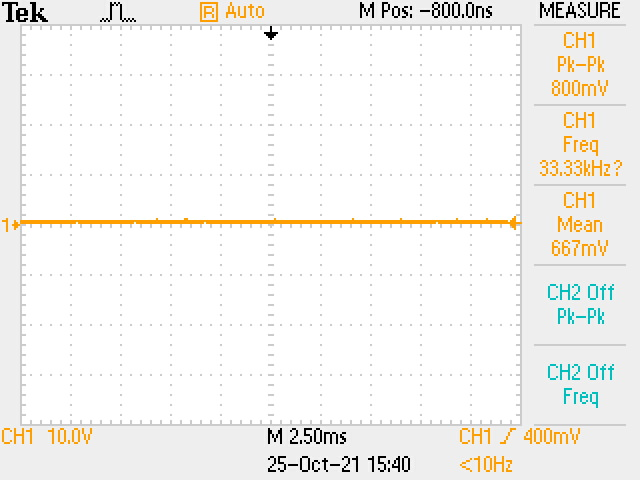
\includegraphics[width=\columnwidth]{img/testing/power_output/filter_output_2kHz.JPG}
      \subcaption{}
  \end{subfigure}
  \caption{}
\end{figure}

\begin{figure}[h!]
  \centering
  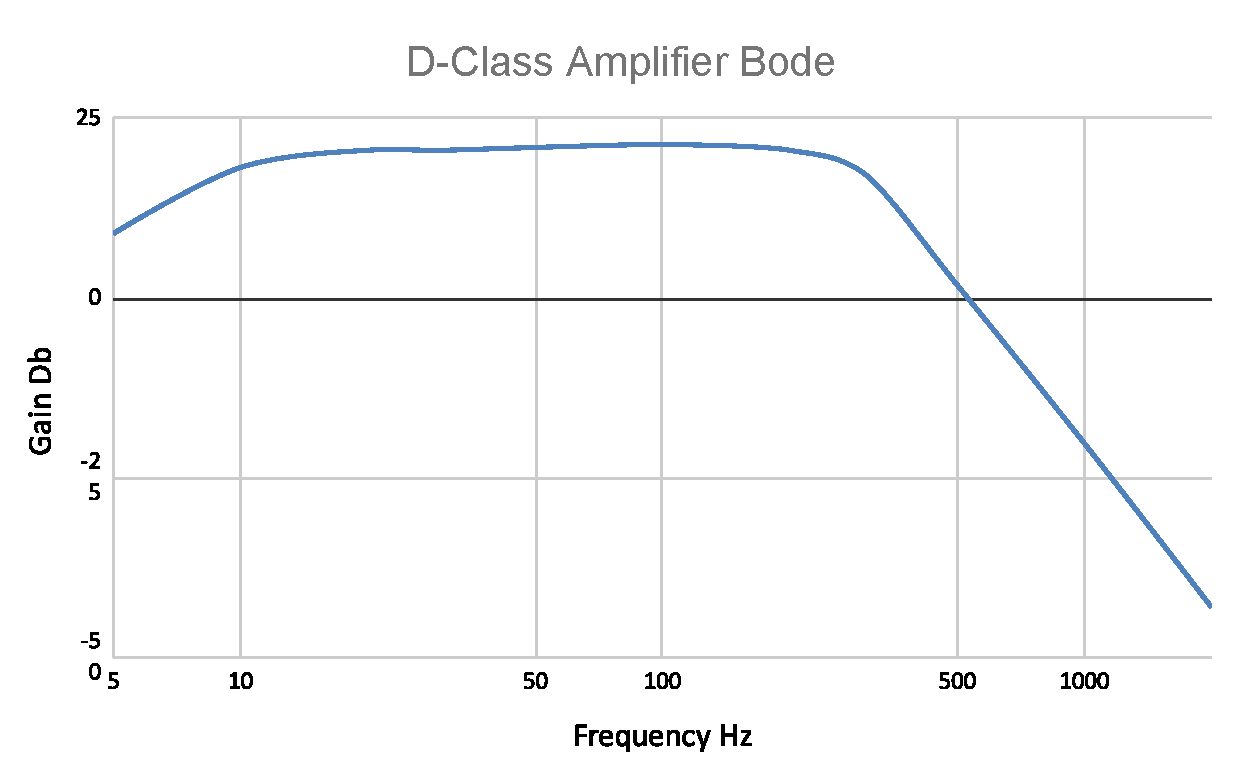
\includegraphics[width=0.75\textwidth]{img/testing/amplifier_bode.pdf}
  \caption{}
\end{figure}

\begin{figure}[h!]
  \centering
  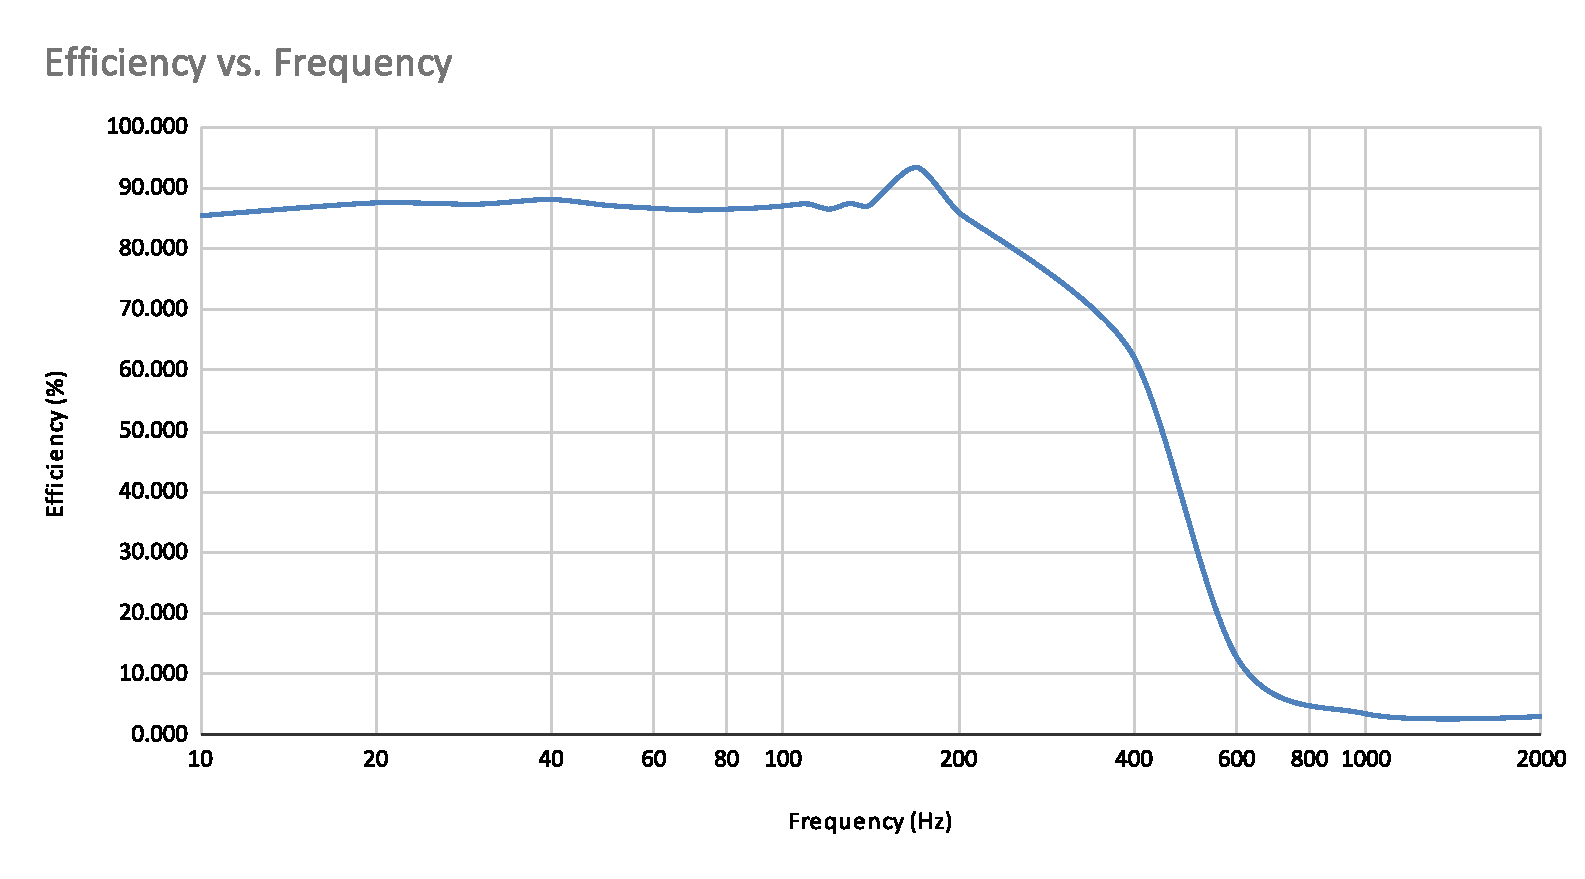
\includegraphics[width=0.75\textwidth]{img/testing/Efficiency_vs._Frequency.pdf}
  \caption{}
\end{figure}

\begin{table}[h!]
  \centering
  \begin{tabular}{l|l}
  \rowcolor[HTML]{E0E0E0} 
  \textbf{Frequency (Hz)} & \textbf{THD (\%)} \\ \hline
  30                 & 1.8               \\
  50                 & 2.2               \\
  100                & 3.2               \\
  200                & 3.3               \\
  300                & 3.5               \\
  500                & 3.2              
  \end{tabular}
  \caption{Output total harmonic distortion across frequency}
  \label{T:THD}
\end{table}


\section{Conclusions}
 
\textit{What worked, didn’t work? How would you change your approach? Any interesting insights?}

Per brd the price was kept to the 50 dollar per mark as per this BOM (https://niels-clayton.github.io/D-Class\_Amplifier/)

\newpage
\section*{Appendix}

\subsection*{Input Filter}
\begin{figure}[h!]
  \centering
  \begin{subfigure}{0.3\textwidth}
    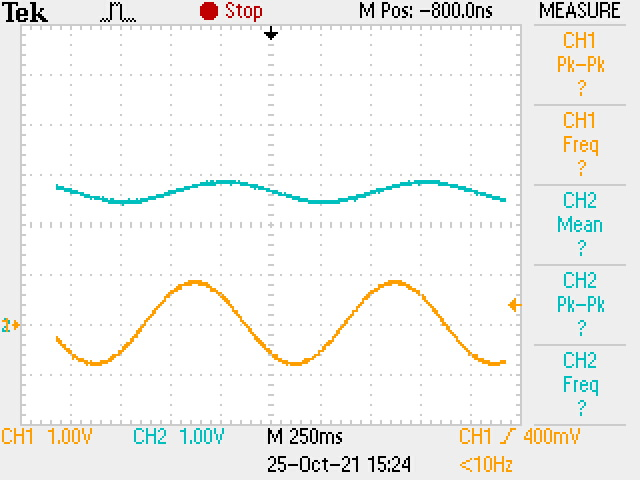
\includegraphics[width=\columnwidth]{img/testing/input_filter/input_1Hz.JPG}
    \subcaption{1Hz}
  \end{subfigure}
  \begin{subfigure}{0.3\textwidth}
    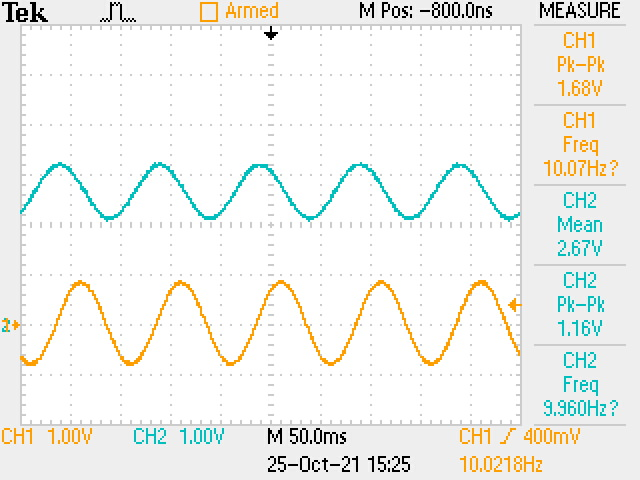
\includegraphics[width=\columnwidth]{img/testing/input_filter/input_10Hz.JPG}
    \subcaption{10Hz}
  \end{subfigure}
  \begin{subfigure}{0.3\textwidth}
    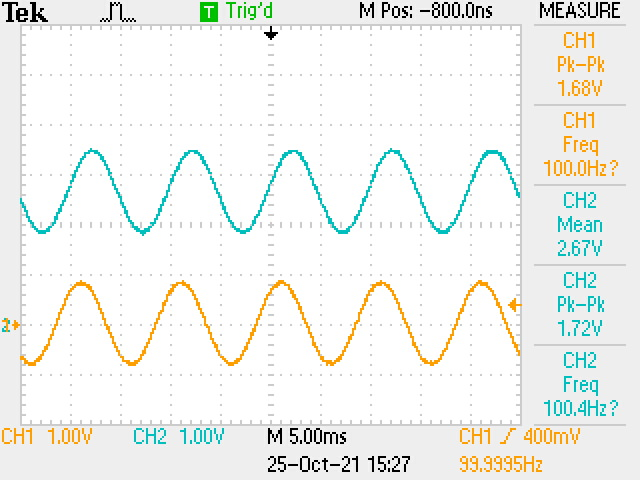
\includegraphics[width=\columnwidth]{img/testing/input_filter/input_100Hz.JPG}
    \subcaption{100Hz}
  \end{subfigure}
  \begin{subfigure}{0.3\textwidth}
    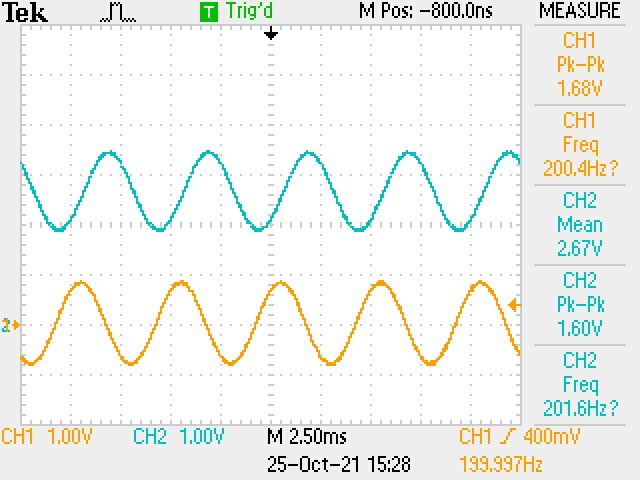
\includegraphics[width=\columnwidth]{img/testing/input_filter/input_200Hz.JPG}
    \subcaption{200Hz}
  \end{subfigure}
  \begin{subfigure}{0.3\textwidth}
    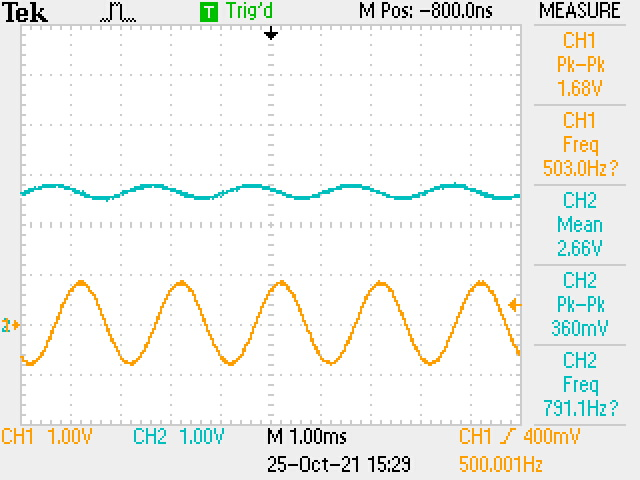
\includegraphics[width=\columnwidth]{img/testing/input_filter/input_500Hz.JPG}
    \subcaption{500Hz}
  \end{subfigure}
  \begin{subfigure}{0.3\textwidth}
    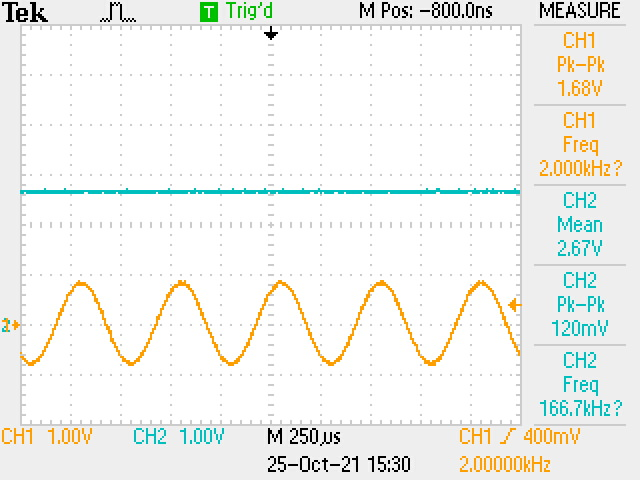
\includegraphics[width=\columnwidth]{img/testing/input_filter/input_2kHz.JPG}
    \subcaption{2kHz}
  \end{subfigure}
\end{figure}

\subsection*{Sampling/SPWM}
\begin{figure}[h!]
  \centering
  \begin{subfigure}{0.3\textwidth}
    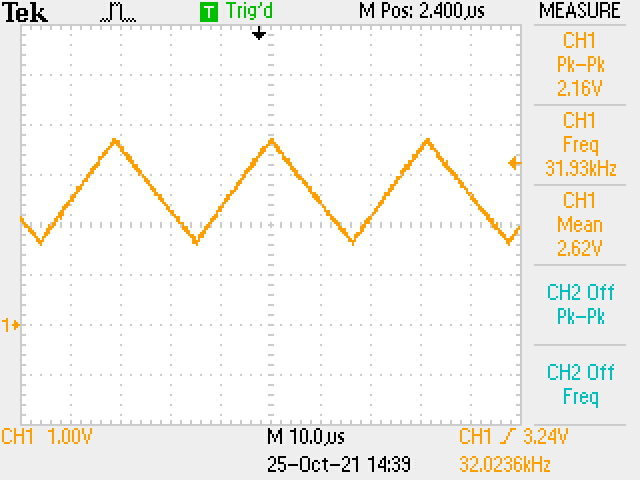
\includegraphics[width=\columnwidth]{img/testing/spwm/triangle_wave_32kHz.JPG}
    \subcaption{Triangle Qave}
  \end{subfigure}
  \begin{subfigure}{0.3\textwidth}
    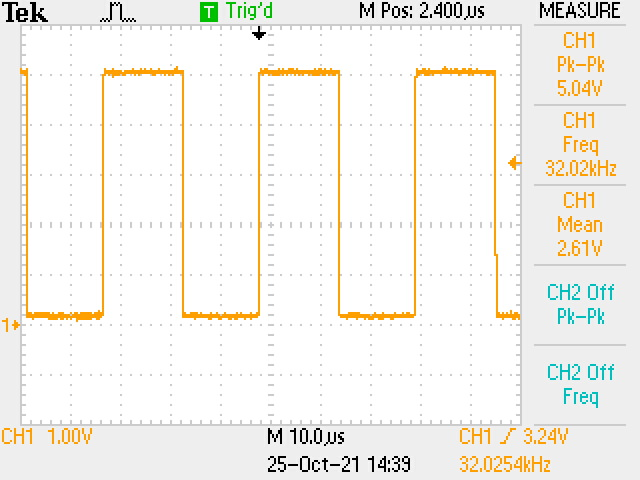
\includegraphics[width=\columnwidth]{img/testing/spwm/spwm_no_input.JPG}
    \subcaption{SPWM w/ 0V Input}
  \end{subfigure}\\
  \begin{subfigure}{0.3\textwidth}
    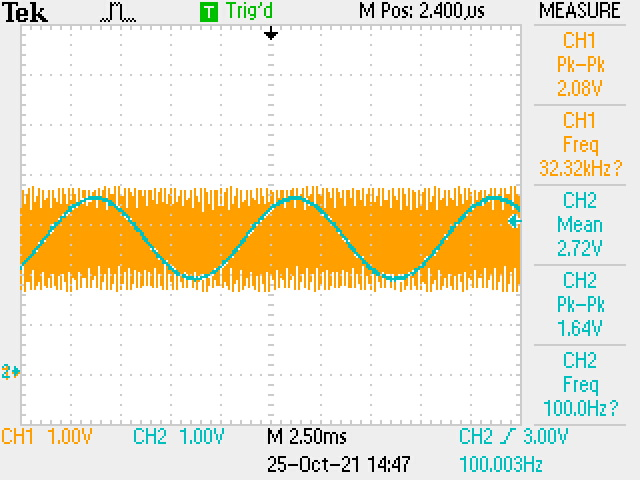
\includegraphics[width=\columnwidth]{img/testing/spwm/input_sampling_0.JPG}
    \subcaption{Input Signal Sampling Far}
  \end{subfigure}
  \begin{subfigure}{0.3\textwidth}
    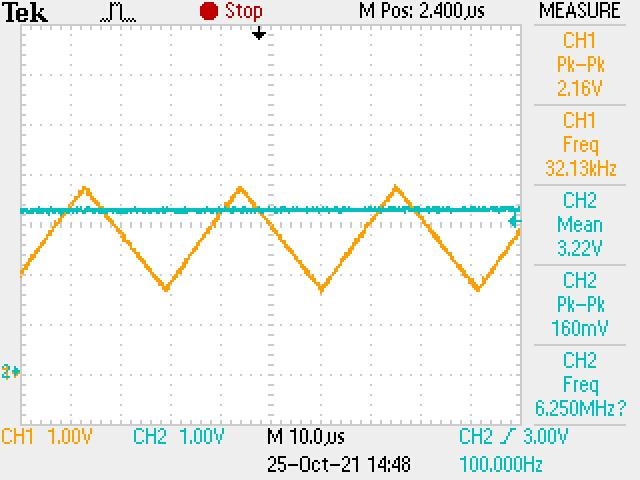
\includegraphics[width=\columnwidth]{img/testing/spwm/input_sampling_1.JPG}
    \subcaption{Input Signal Sampling Near}
  \end{subfigure}
\end{figure}

\end{document}